\chapter{Introduzione}

Il corso si divide in una serie di sezioni:
\begin{itemize}
    \item [$\Rightarrow$] Macchine mai esistite (Knowledge
    Navigator, Dynabook, Memex): poichè la storia dell'informatica
    è una storia di idee, di pionieri e di visionari;
    \item [$\Rightarrow$] Il modo di organizzare i testi in rapporto all'inondazione 
    informativa: workstation di Otlet (non realizzata), the mother of all
    demos (Doug Engelbart, 1968), gli ipertesti di Ted Nelson, libraries
    of the future;
    \item [$\Rightarrow$] La cybernetica: originata da Norbert Wiener, ci si concentra sugli
    aspetti matematici della neurofisiologia che portarono al modello formale di
    neurone (McCulloch e Pitts, 1943) utilizzato da Von Neumann per la
    definizione della sua architettura di calcolatore;
    \item [$\Rightarrow$] Gli hippies e la controcultura: si parla di come la controcultura 
    abbia influenzato la nascita dell'informatica;
    \item [$\Rightarrow$] La semiotica: si parte in ordine cronologico dalla preistoria, passando per Lullo fino
    a Leibniz, per arrivare ai sistemi formali.
\end{itemize}

\section{La preistoria dell'informatica}

\qs{}{Perchè studiare cosi indietro nel tempo?}

\paragraph{Risposta:} perchè si vuole caratterizzare il
concetto di calcolo e si vogliono comprendere le abilità cognitive
su cui tale concetto si basa.

\subsubsection{}

Circa 110.000 anni fa si ha, in Cina, il primo esempio di astrazione con degli \newfancyglitter{ossi intagliati}. Essa è la produzione consapevole di una traccia relativamente stabile. Successivamente, intorno al 8000 a. C., sono stati usati dei \newfancyglitter{gettoni} in argilla. Presumibilmente questa è la nascita simultanea della scrittura e del calcolo. I gettoni vennero affiancati dalle \newfancyglitter{tavolette d'argilla}, modellate usando dei calchi (come un rudimentale libro contabile).

\paragraph{I gettoni:}

\begin{itemize}
    \item [$\Rightarrow$] Favoriscono la raccolta di dati;
    \item [$\Rightarrow$] Sono immediati da comprendere;
    \item [$\Rightarrow$] Permettono le operazioni aritmetiche come manipolazioni concrete.
\end{itemize}

Un ulteriore fenomeno è quello delle \newfancyglitter{bolle} che contengono dei gettoni. Venivano usate come registrazione di un contratto quando un proprietario di bestiame dava in affitto la sua mandria per la transumanza.

Oltre agli strumenti d'argilla vennero usati dei \newfancyglitter{bastoncini di legno} che venivano divisi in due metà: una ricevuta e un titolo di credito. Il titolo di credito si chiamava \newfancyglitter{stock} (da qui il termine "stock market") e la ricevuta si chiamava stub.

\subsection{Semiotica}

Nei meccanismi illustrati nella sezione precedente i segni hanno un ruolo importante. 

\dfn{Semiotica}{La \newfancyglitter{semiotica} è la scienza che studia i linguaggi e i segni che li costituiscono.}

\cor{Il linguaggio}{In ogni linguaggio sono presenti tre componenti:

\begin{itemize}
    \item [$\Rightarrow$] Chi produce i segni (studiati dalla pragmatica);
    \item [$\Rightarrow$] I segni prodotti (studiati dalla sintassi);
    \item [$\Rightarrow$] Il significato dei segni (studiati dalla semantica).
\end{itemize}
}
\paragraph{}

La semiotica è direttamente collegata all'informatica (computer semiotics):

\begin{itemize}
    \item [$\Rightarrow$] Un computer è spesso utilizzato per generare, trasformare e visualizzare segni (il PC come medium);
    \item [$\Rightarrow$] Un computer viene programmato utilizzando un linguaggio.
\end{itemize}

\newfancyglitter{Kenneth Iverson} fu un importate semiotico e fu il fondatore del linguaggio esoterico APL, che nacque come linguaggio logico. APL influenzo molti linguaggi funzionali, come Haskell, e il paradigma di parallelismo.

\begin{center}
    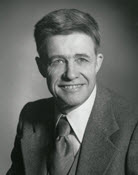
\includegraphics[scale = 1]{images/iverson.jpg}
\end{center}


\section{Leibniz}

Nasce a Lipsia il 21 Giugno 1646, si laurea in Giurisprudenza nel 1666.
I suoi primi scritti sono finalizzati al conseguimento di titoli accademici. Importante in
questo periodo è la Dissertatio de Arte Combinatoria del 1666.
Negli anni immediatamente successivi alla laurea diventa consigliere dell’Elettore di
Magonza ed assume diversi incarichi politici.

\begin{center}
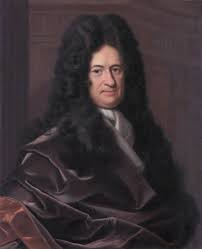
\includegraphics[scale = 0.7]{images/Leibniz.jpg}
\end{center}

Nel 1672 viene inviato a Parigi in missione diplomatica, per distogliere Luigi XIV dalla
progettata invasione dell’Olanda ed invogliarlo invece alla conquista dell’Egitto.
Fallita la missione, ottiene il permesso di fermarsi a Parigi (e Londra), dove rimane per 4
anni (marzo 1672-ottobre 1676) avendo la possibilità di conoscere la matematica e la
fisica più avanzate. Nel 1676 scopre il calcolo infinitesimale (che verrà pubblicato solo ne 1684), già
introdotto da Newton indipendentemente 10 anni prima. Nel 1705 inizierà tra i due una
polemica che finirà solo con la morte di Leibniz.
Nello stesso anno torna ad Hannover come bibliotecario presso il Duca di Hannover.

Tra il 1685 e il 1694: migliora la scatola di Pascal (\newfancyglitter{pascalina}) per l’addizione e la sottrazione per realizzare
anche la moltiplicazione e la divisione (e l’estrazione di radice). La macchina, che opera
mediante pulegge e ruote dentate, è conservata nella biblioteca di Hannover.

\subsection{L'origine del bit}

Leibniz fece un parallelismo tra i simboli dello yin e dello yang e i numeri binari.
Le linee piene potevano essere associate al 1, mentre le linee vuote al 0.
Così facendo si ottiene un sistema di numerazione binario.

\begin{center}
    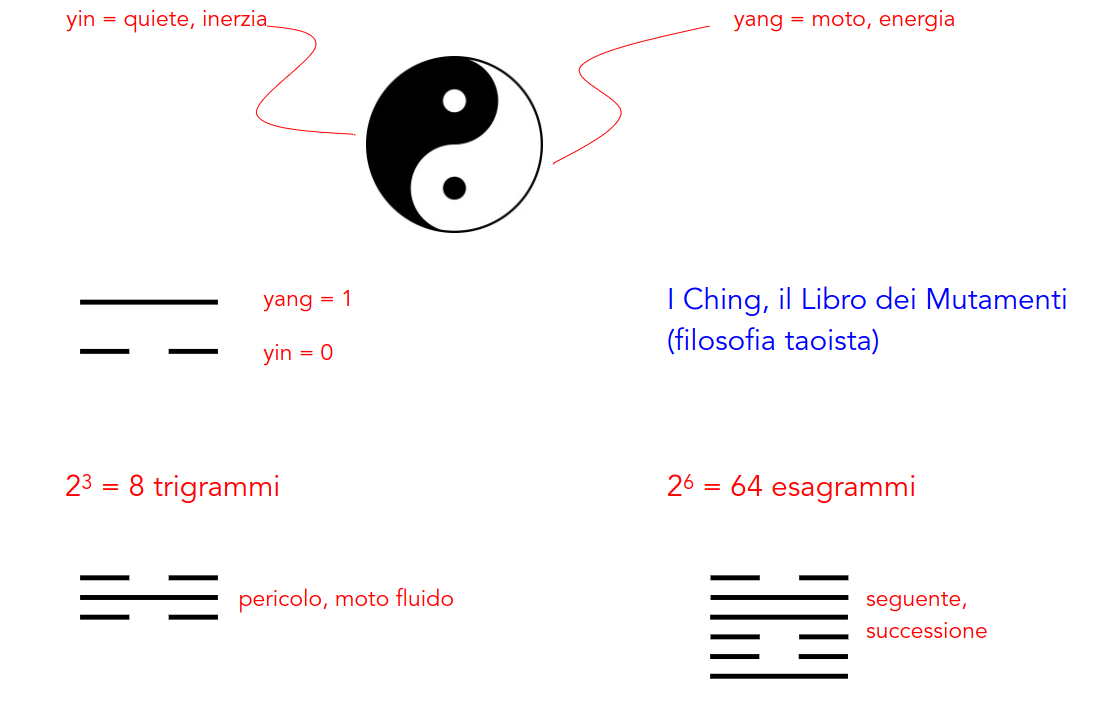
\includegraphics[scale = 0.3]{images/Origine bit.png}
\end{center}

\pagebreak

\ex{L'interpretazione di Leibniz}{
    \begin{center}
        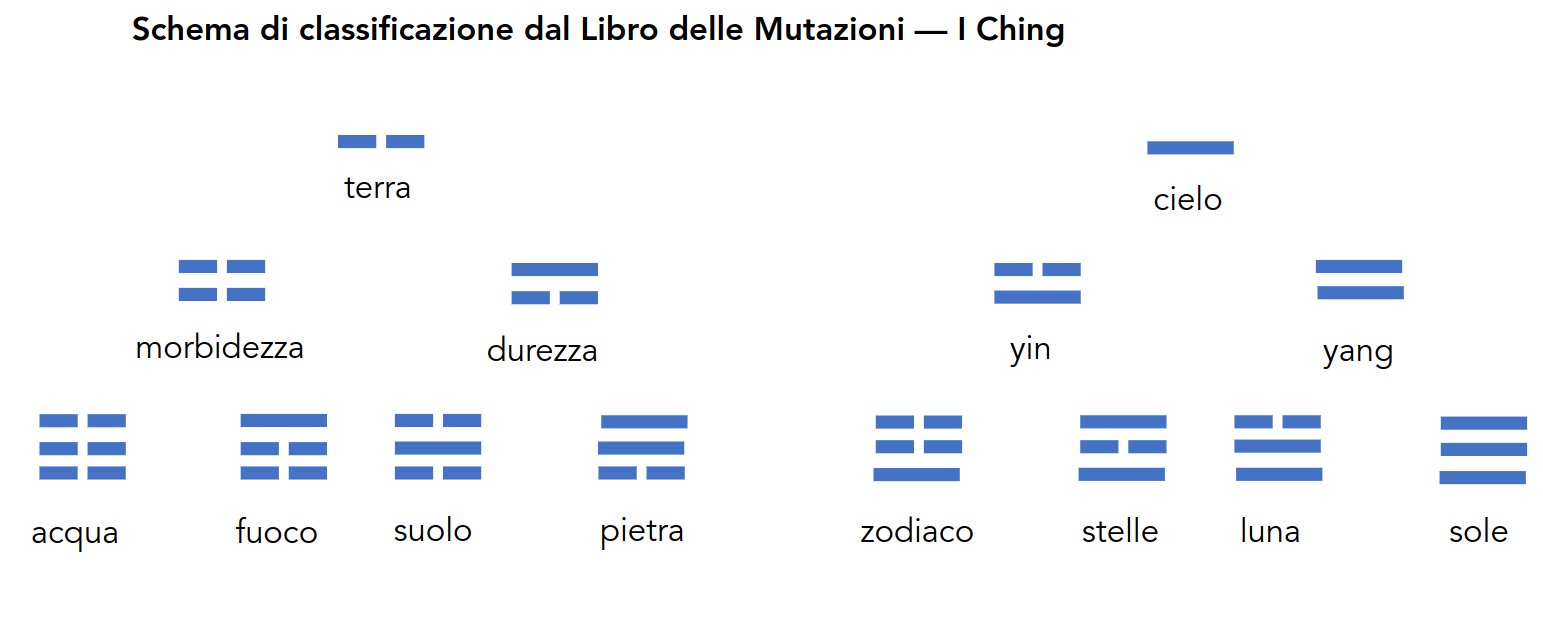
\includegraphics[scale = 0.27]{images/Bit.png}
        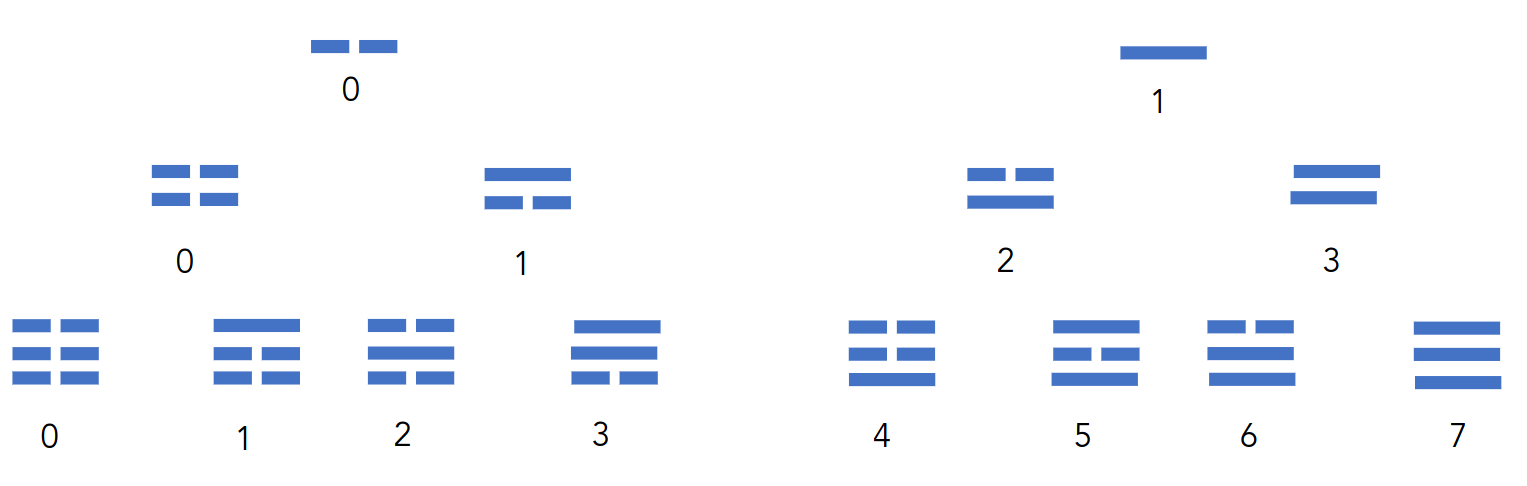
\includegraphics[scale = 0.27]{images/Associazione di Leibniz.png}
    \end{center}
}

\subsection{La caratteristica universale}

La \newfancyglitter{caratteristica universale}, concepita come lingua o scrittura universale, si fonda sui seguenti principi:

\begin{itemize}
    \item [$\Rightarrow$] Le idee sono analizzabili fino a idee semplici (atomiche);
    \item [$\Rightarrow$] Le idee possono essere rappresentate da simboli;
    \item [$\Rightarrow$] Le relazioni tra idee possono essere rappresentate da simboli;
    \item [$\Rightarrow$] Le idee si combinano mediante regole.
\end{itemize}

\dfn{Caratteristica universale}{
La \newfancyglitter{caratteristica universale} è un sistema di segni che rappresentano
nozioni e cose, ma non parole. Le connessioni tra i segni rappresentano le relazioni tra le nozioni e le cose.
Il nome di una nozione serve a:
\begin{itemize}
    \item [$\Rightarrow$] Relazionarla con altre nozioni;
    \item [$\Rightarrow$] Relazionarla con lo schema dell'universo;
    \item [$\Rightarrow$] Indicare le esperienze necessarie per la conoscenza.
\end{itemize}
}

\nt{L'apprendimento della lingua universale coincide con l'\fancyglitter{enciclopedia}. }


\subsubsection{Il calculus ratiocinator}

\dfn{Calculus ratiocinator}{Il \newfancyglitter{calculus ratiocinator} è un insieme di tecniche per manipolare i segni della caratteristica universale. Può essere considerato come un \newfancyglitter{sistema formale}. Il frammento XX offre un'idea di questo calcolo: in esso vengono trattati molti assiomi e teoremi come il principio degli indiscernibili, la simmetria, la transitività, etc.}

\subsection{La mereologia}

\dfn{Mereologia}{
    La \newfancyglitter{mereologia} è la "dottrina delle parti".
}

\dfn{Principio di identità degli indiscernibili}{
    Soo identici i termini che possono essere sostituiti a vicenda
    senza alterare la verità degli enunciati in cui compaiono. Si scrive A = B 
    quando A e B sono identici.
    \begin{itemize}
        \item [$\Rightarrow$] $B + N = L$ significa che B e N compongono L,
        cioè che B è parte di L;
        \item [$\Rightarrow$] $A\leq B$ significa che A è parte di B.
    \end{itemize}
}

\thm{Simmetria}{
    Se $A = B$ allora $B = A$.
}

\thm{Transitività}{
    Se $A = B$ e $B = C$ allora $A = C$.
}

\thm{}{
    Se $A + B = B$ allora $A \leq B$.
}

\thm{}{
    Se $A = B$ allora $A + L = B + L$.
}
\pagebreak
\section{Peano}

Peano nacque a Cuneo il 27 agosto 1858. Si laureò in matematica nel 1880 e divenne professore di analisi matematica a Torino nel 1890. Nel 1889 pubblicò i suoi famosi \newfancyglitter{Principi di aritmetica}, in cui formulò un sistema assiomatico per i numeri naturali.

\begin{center}
    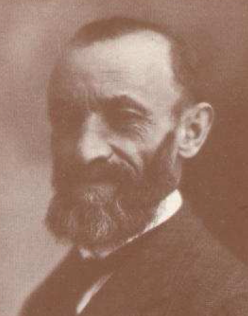
\includegraphics[scale = 0.7]{images/Peano.png}
\end{center}

\dfn{Principi di aritmetica}{
    I \newfancyglitter{Principi di aritmetica} sono un insieme
    di assiomi che definiscono i numeri naturali.
}

\subsection{Sistemi formali}

\nt{Sono trattati più in dettaglio nel corso "Metodi formali dell'Informatica" e, in
misura minore, nel corso di "Linguaggi e paradigmi di programmazione".}

\dfn{Sistema formale}{
    In un \newfancyglitter{sistema formale} si definiscono:
    \begin{itemize}
        \item [$\Rightarrow$] \fancyglitter{Oggetti}, che sono tutti i termini costruibili a partire 
        da atomi mediante operazioni;
        \item [$\Rightarrow$] \fancyglitter{Proposizioni}, della forma $P(a_1, ..., a_n)$ dove
        $P$ è un \fancyglitter{predicato} e $a_k$ sono termini;
        \item [$\Rightarrow$] \fancyglitter{Regole di inferenza}, che permettono di dedurre nuove proposizioni.
        La conclusione di una regola di inferenza senza premesse è un'\fancyglitter{assioma}.
    \end{itemize}

    $$\frac{A_1 \:\:\:\:\:\:\:\:\:...\:\:\:\:\:\:\:\:\: A_v}{A}$$
}

\qs{}{Come si usano le regole di inferenza?}

\paragraph{Risposta:} Per costruire derivazioni: $$\frac{\frac{
    A_1 \:\:\:\:\:\:\:\:\:\:\:\:\:\:\:\:\:\: A_2}{A}\:\:\:\:\:\:\:\:\: B}{C}$$

\ex{Numeri naturali}{
    \begin{itemize}
        \item [$\Rightarrow$] \fancyglitter{Oggetti}: un atomo 0, un'operazione S, con un solo argomento;
        \item [$\Rightarrow$] \fancyglitter{Proposizioni}: un predicato Num con un solo argomento;
        \item [$\Rightarrow$] \fancyglitter{Regole di inferenza}: $\frac{}{\text{Num\{0\}}}$ e 
        $\frac{\text{Num\{n\}}}{\text{Num\{S(n)\}}}$.
    \end{itemize}
}